\documentclass[a4paper]{article}
\usepackage[font=small,labelfont=bf]{caption}
\usepackage[T1]{fontenc}
\usepackage[utf8]{inputenc}
\usepackage[italian]{babel}
\usepackage{url} % per scrivere gli indirizzi url
\usepackage{booktabs}
\usepackage{graphicx}
\usepackage[left=1.5cm,bottom=1.5cm,right=1cm,top=1cm]{geometry}
\usepackage{frontespizio}
\usepackage{wrapfig}
\usepackage{xcolor}
\usepackage{color}
\usepackage{siunitx}  
\usepackage{hyperref}
\usepackage{listings}
\usepackage{framed} %linee nel lsting
\usepackage{parskip} %risolve i dannati indent.
\usepackage{fancyvrb}





\definecolor{comment}{RGB}{237, 141, 33}
\definecolor{backy}{RGB}{ 255, 253, 183 }
\definecolor{back}{RGB}{ 30,30,30 }
\definecolor{shadecolor}{RGB}{ 30,30,30 }
\lstset{
%rulecolor=\color{white},
numbers=left,
numberstyle=\color{black},
%backgroundcolor=\color{back},   
frame=single,
showspaces=false,
basicstyle=\ttfamily,%\color{white},
showstringspaces=false,
keywordstyle=\color{purple},       % keyword style
commentstyle=\color{comment},    % comment style
stringstyle=\color{blue}    % string literal style
}



\begin{document}

\begin{frontespizio}
%\Universita{Bergamo}
%\Facolta{Pennutologia}
%\Corso{Belle Lettere}
%\Annoaccademico{2030--2031}
%\Titoletto{Tesi di laurea magistrale}
%\Titolo{Relazione di Robotica}
%\Sottotitolo{Alcune considerazioni mutevoli}
%\Candidato[PP999999]{Paperon de' Paperoni}
%\Relatore{Giovanni Episcopo}
%\Relatore{Pippo Cluvio}
%\Correlatore{Ugo Frogio}
%\Correlatore{Ubaldo Kutuzu}

\end{frontespizio}
\tableofcontents
\newpage

    

\section{ROS per NVIDIA Jetson TX2}
Questa parte del progetto ha richiesto l'installazione e la configurazione dell'ambiente ROS sulla scheda Jetson TX2.
Tra le operazioni preliminari è stata effettuata l'installazione di L4T (linux for tegra) sulla scheda per fornire kernel,driver,librerie e un sistema operativo
correttamente configurato per l'architettura specifica della Jetson.

\subsection{Setup tramite tool Jetpack}
La scheda é dotata di pulsanti per il controllo diretto, per l'accensione della scheda é necessario premere il tasto contrassegnato sulla pcb con il label 'POWERBTN'.\\
La scheda inizialmente necessita di un flash tramite un tool chiamato 'JetPack' scaricabile dal sito nvidia da eseguire su un pc dotato di porta usb.\\
Come prima cosa collegare la Scheda Jetson a internet attraverso un cavo ethernet connesso allo stesso router del pc su cui eseguiremo Jetpack mantenendo la scheda spenta.
Sulla scheda sono presenti 4 tasti rossi evidenziati da un riquadro rosso nella \ref{fig:jetsonTX2} che,dall'alto al basso, sono: RESET,VOL-,RECOVERY,POWER ON/OFF.\\
Avviare la scheda jetson in 'recovery mode' seguendo questa sequenza di operazioni:\\
\vspace{-10pt}
\begin{wrapfigure}{r}{0.35\textwidth}
    \centering
    
    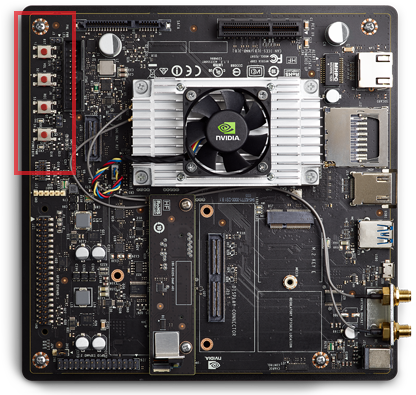
\includegraphics [width=0.3\textwidth] {NVIDIA_Jetson_TX2_Module_Devkit.png}
   
    \caption{Jetson TX2.}
    \label{fig:jetsonTX2}
\end{wrapfigure}
\begin{enumerate} 
    \item accendere la scheda premendo il pulsante di POWER ON/OFF .
    \item tendo premuto il pulsante RECOVERY premere e rilasciare il pulsante RESET.
    \item rilasciare dopo 2 secondi dalla pressione del pulsante RESET il pulsante RECOVERY.
    \item Collegare il cavo micro usb B alla scheda e l'altra estremitá ad una porta usb sul pc su cui si eseguirá jetpack. 
\end{enumerate}
Una volta scaricato l'archivio dal sito ufficiale e estratto in una cartella su un pc (non quindi sulla jetson) avviare da terminale (le istruzioni sono per S.O. linux)
il file eseguibile 'Jetpack-L4T-versione-linux-x64.run' tramite il comando './Jetpack-L4T-versione-linux-x64.run', seguire le istruzioni del'interfaccia che si presenterá a video
per selezionare cartella di installazione, modello della scheda e selezione dei pacchetti che si desidera installare sulla jetson quali openCV e il toolkit CUDA.
Accettare eventualmente i termini e le condizioni d'uso una volta premuto 'Next'.
Nella scheda 'Network layout' selezionare la scelta coerente con la configurazione di rete attuale della nostra scheda ovvero la prima ('Device access internet via router/switch').
Selezionare la propria interfaccia di rete connessa a internet (nel dubbio utilizare il comando da terminale 'ifconfig' e cercare a quale interfaccia di rete è assegnato un indirizzo IPv4).
Dopo la schermata riassuntiva, alla pressione del tasto next si presenterá una finestra del terminale per visualizzare i progressi dell'installazione.
In caso di errori relativi al collegamento della jetson ripetere la sequenza di operazioni per porla in recovery mode.


\subsection{Backup e ripristino}
Una volta eseguito jetpack e scaricate le dipendenze verranno creati in specifiche cartelle script per eseguire operazioni manualmente sulla jetson
quali backup e ripristino ad esempio.\\
Per fare ciò navighiamo nella cartella contenente L4T (nel mio calcolatore la directory era '64\char`_TX2/Linux\char`_for\char`_Tegra') dove sarà presente il file 'flash.sh'.\\
Apriamo dunque un terminale in questa posizione e colleghiamo la scheda al pc in modalità recovery.

\subsubsection{Backup}
Utilizzare il comando "sudo ./flash.sh -r -k APP -G backup.img jetson-tx2 mmcblk0p1" che eseguirà il backup di tutta la memoria dell'emmc da 30Gb della scheda
generando due files 'backup.img' e 'backup.img.raw' entrabi da conservare.

\subsubsection{Ripristino}
Per ripristinare un backup posizionare il "backup.img" nella directory contenente flash.sh e copiare il file backup.img.raw nella cartella bootloader rinominandolo system.img.
Aprire ora un terminale nella cartella contenente flash.sh e digitare "sudo ./flash.sh -r -k APP jetson-tx2 mmcblk0p1" , questo comando si occuperà di eseguire il flash della partizione p1 del disco mmcblk0 (l'emmc della scheda.)\\

\newpage
\subsection{Possibile errore}
\begin{figure}[h]
    \centering
    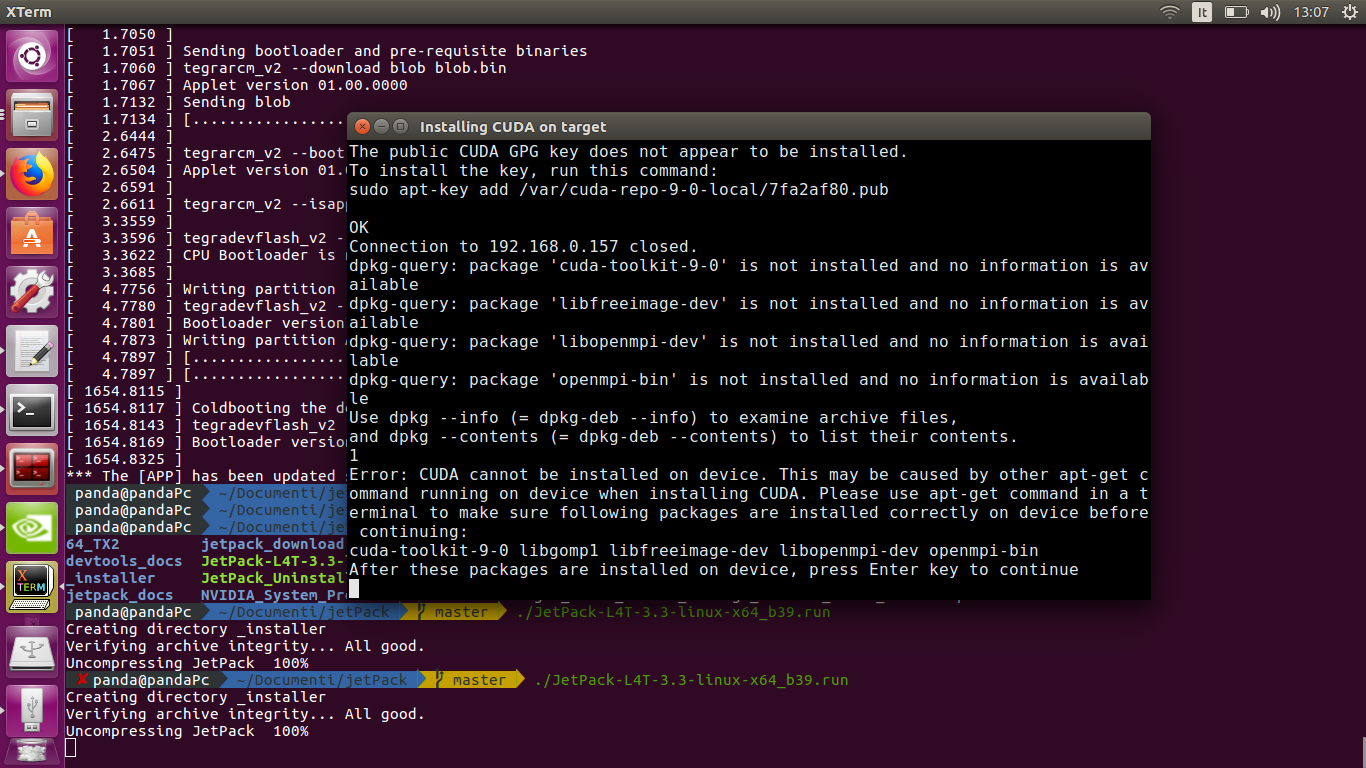
\includegraphics[width=10cm]{err1.png}    
    \caption{errore durante il flash.}
    \label{fig:err1}
\end{figure}
Nella mia personale esperienza si è verificato un errore durante il flash della scheda dovuto all'interruzione della connessione internet, probabilmente causato 
da filtri sulla rete universitaria o a una momentanea instabilitá della connessione. Per risolvere il problema ho collegato la tastiera alla scheda jetson,ho installato manualmente i pacchetti mancanti tramite apt-get e infine premuto enter come indicato da jetpack nel terminale sul mio pc personale (n.b. eseguire "sudo apt-get update" sulla jetson prima di qualsiasi apt-get install per aggiornare le repositories)

\subsection{Setup di Ubuntu}
\subsubsection{Setup tastiera}
Avviato ubuntu il layout di tastiera potrebbe essere errato, per cambiarlo digitare in un terminale 'sudo dpkg-reconfigure keyboard-configuration':
\begin{enumerate}
    \item accettare 'Generic 105-key (intl) PC'
    \item selezionare Italian nel menù del paese di origine della tastiera
    \item accettare le restanti impostazioni senza modificarle
\end{enumerate}
\subsubsection{Installazione ros}
Seguire le indicazioni per l'istallazione di ros-kinetic dal \href{http://wiki.ros.org/action/show/kinetic/Installation/Ubuntu?action=show&redirect=kinetic%2FInstallation%2FUbuntuARM}{\underline{\color{blue}{sito ufficiale per ubuntu ARM.}}}
\newpage

\section{ROS: COMUNICAZIONE SERIALE TRAMITE USB}
Per interfacciarsi con board quali arduino tramite ros è risultato necessario un metodo per la comunicazione seriale tramite porta USB per poter ricevere e inviare dati in modo semplice e efficace.
Tale metodo è stato sviluppato pensando ad un utilizzo con board arduino su macchina linux e sviluppato in C++ per essere compatibile con ROS.
Tutte le board arduino sono dotate di un chip UART ( Universal asynchronous receiver-transmitter) incaricato della comunicazione seriale.
Il metodo di comunicazione asincrono si basa sull'invio di dati a una velocitá predefinita e con dati strutturati in modo ben preciso:
\begin{enumerate} 
    \item Bit contenenti parte del messaggio complessivo di grandezza predefinita (dai 5 ain 9 in base alle impostazioni)
    \item Bit di sincronizzazione per comunicare l'inizio e la fine di ciascun pacchetto di dati.
    \item Bit di paritá per il controllo di errori
    \item velocitá di trasmissione dei dati per impostare su ogni singolo invio la velocitá di invio e ricezione.
\end{enumerate}
Sono state sperimentate diverse librerie per la comunicazione seriale e metodi basati su programmazione seriale per sistemi POSIX per scegliere infine la libreria boost per la sua semplicitá e per la documentazione online relativamente completa.
Il codice scritto per la comunicazione è il seguente:
\lstinputlisting[language=C++]{SerialIO.h}

Le funzioni di read e write nella comunicazione asincrona stabilita sono bloccanti pertanto la coordinazione dei messaggi deve essere fatta a monte e non viene gestita dal programma.
Questa libreria espone i due metodi di read e write e necessita di un inizializzazione tramite il path del file che punta al dispositivo hardware nella cartella /dev/ (ad esempio un path valido puo essere "/dev/tty1").
Il punto chiave della funzione read si trova alla riga 37 dove viene invocata la funzione di lettura dalla libreria boost:

\begin{lstlisting}[language=C++,firstnumber=37]
read_size=m_port.read_some(boost::asio::buffer(read_msg_,BUFFSIZE));
\end{lstlisting}

La funzione read\_some legge in modo asincrono parte del messaggio, lo copia nel buffer creato ad hoc dal nome read\_msg\_ e di dimensione BUFFSIZE, ritornando la dimensione del messaggio letto.
Il ciclo while successivo serve per giungere al finestringa e copiare in uno stringstream il contenuto dei vari pacchetti del messaggio asincrono.

\begin{lstlisting}[language=C++,firstnumber=38]
while(read_msg_[read_size-1]!='\n')
\end{lstlisting}
Viene ripetuta la lettura fino a quando non viene trovato come ultimo carattere letto il terminatore.Si presuppone quindi che il codice inviato tramite arduino comunichi con una println sulla seriale o che sia inserito il terminatore di stringa manualmente al termine di un messaggio con una semplice print.

\begin{lstlisting}[language=C++,firstnumber=39]
read_msg_[read_size]=0;
ss<<read_msg_;
\end{lstlisting}
Poichè il buffer creato da asio risultava essere non vuoto la copia del buffer nello stringstream senza aggiungere il terminatore manualmente generava stringhe errate, la riga 39 ovvia a questo problema.

\begin{lstlisting}[language=C++,firstnumber=45]
std::cout << ss.str();
\end{lstlisting}

Il messaggio viene stampato sullo standard output utilizzando la funzione di conversione da stringstream a stringa. Questa parte del codice puo essere modificata per eventualmente effettuare un post in un topic ros.
\\
La funzione write è piuttosto simile alla read:

\begin{lstlisting}[language=C++,firstnumber=21]
const int BUFFSIZE=20;	
boost::array<char,BUFFSIZE> buf;
\end{lstlisting}
Viene creato un buffer di dimensione massima 20 (buffer troppo grossi rallentano notevolmente il programma e causano blocchi,ho trovato 20 un numero adeguato ma il valore puo essere modificato secondo necessità).

\begin{lstlisting}[language=C++,firstnumber=24]
for(int i=0;i<sizeof(input)/8;i++){		
    buf[i]=input[i];
}
\end{lstlisting}
La stringa fornita come input viene copiata nel buffer, il ciclo for è stato usato per l'impossibilità di usare funzioni quali strcpy o alternative piu efficienti.

\begin{lstlisting}[language=C++,firstnumber=27]
buf[sizeof(input)/8]=0;
\end{lstlisting}
Viene aggiunto manualmente un terminatore nel buffer onde evitare errori.

\begin{lstlisting}
m_port.write_some(boost::asio::buffer(buf,sizeof(input)));
\end{lstlisting}
Viene inviato il messaggio contenuto nel buffer specificando la dimensione del messaggio da inviare.
\newpage
Per una piu facile inizializzazione della comunicazione seriale è stato scritta una libreria sempre in C++ per trovare un Arduino e ritornare il path del suo riferimento necessario per l'inizializzazione.


\lstinputlisting[language=C++,title=\lstname]{deviceFinder.h}
\lstinputlisting[language=C++,title=\lstname]{finder.o}
La libreria deviceFinder.h sfrutta lo script per la bash finder.o per ricavare la stringa desiderata.
È importante notare che il programma finder.o deve avere le autorizzazioni per essere eseguito (chmod +x finder.o) e deve essere eseguito su un sistema Linux.
Lo script finder.o elenca semplicemente path dei device connessi e relativi id caratteristici:
\lstinputlisting[language=C++,title=\lstname,firstline=8,lastline=8]{finder.o}
Il programma in C esegue quindi lo script e tramite piping nella shell filtra il risultato avente "Arduino" come stringa nel vendor id e prende il primo token della stringa:
\lstinputlisting[language=C++,title=\lstname,firstline=13,lastline=13]{deviceFinder.h}
La stringa viene dunque copiata e l'indirizzo isolato viene restituito dalla funzione getArduino().
La libreria può dunque essere usata con la classe SerialIO per cercare automaticamente la porta a cui è connesso il device Arduino e inizializzare al comunicazione seriale nel seguente modo:
\begin{lstlisting}[language=C++]
#include "SerialIO.h"
#include "deviceFinder.h"
int main(int argc, char* argv[]){
    SerialIO arbitrary_name(getArduino());
    arbitrary_name.write("something");
    arbitrary_name.read();
}
\end{lstlisting}

\newpage




\section{ZED}
Lo ZED è una fotocamera che riproduce il modo in cui funziona la visione umana. Usando due sensori RGB da $4MP$ e attraverso la triangolazione, la ZED fornisce una comprensione tridimensionale della scena che osserva, permettendo al robot di diventare consapevole dello spazio e del movimento.


Cattura video 3D ad alta definizione , fino a $2K $ , con un ampio campo visivo ($\ang{110}$) e apertura $f/2.0$. La camera genera due flussi video destro e sinistro sincronizzati in formato side-by-side su USB 3.0. \'E disponibile la retrocompatibilità con USB 2.0.
\\
\\
Sono disponibili diverse modalità video:
\begin{center}
\begin{tabular}{llll}
\toprule
Modalità video &Risoluzione di uscita (affiancata) &	Frame Rate (fps) &	Campo visivo \\
\midrule
2.2K&	4416x1242&	15	 &Largo \\
1080p	&3840x1080&	30, 15&	Largo\\
720p&	2560x720&	60, 30, 15&	Extra largo\\
WVGA&	1344x376&	100, 60, 30, 15&	Extra largo\\
\bottomrule
\end{tabular}
\end{center}
Lo ZED emette le immagini in diversi formati. 
\'E possibile selezionare tra immagini rettificate, non rettificate e in scala di grigi.
\paragraph{Profodità}
Lo ZED riproduce il funzionamento della visione binoculare umana. Gli occhi umani sono separati orizzontalmente di circa 65 mm in media. Quindi, ogni occhio ha una visione leggermente diversa del mondo circostante. Confrontando queste due viste, il nostro cervello può inferire non solo la profondità ma anche il movimento 3D nello spazio. Allo stesso modo, lo ZED ha due occhi separati da 12 cm che catturano un video 3D ad alta risoluzione della scena e stimano profondità e movimento confrontando lo spostamento dei pixel tra le immagini sinistra e destra.
\paragraph{Mappa di profondità}
Lo ZED memorizza un valore di distanza (Z) per ciascun pixel (X, Y) nell'immagine. La distanza è espressa in  metri e calcolata dal retro dell'occhio sinistro della telecamera all'oggetto della scena.

Le mappe di profondità catturate dallo ZED non possono essere visualizzate direttamente poiché sono codificate su 32 bit. Per visualizzare la mappa di profondità, è necessaria una rappresentazione monocromatica (in scala di grigi) a 8 bit con valori compresi tra [0, 255], dove 255 rappresenta il valore di profondità più vicino possibile e 0 il valore di profondità più distante possibile.
\paragraph{Mappatura 3D}
La ZED scansiona continuamente i suoi dintorni e crea una mappa 3D di ciò che vede. Questa mappa viene aggiornata quando il dispositivo viene spostato acquisendo nuovi elementi nella scena. Poiché la fotocamera percepisce le distanze oltre la gamma dei tradizionali sensori RGB-D, è in grado di ricostruire rapidamente mappe 3D di grandi aree interne ed esterne.

\subsection{ZED SDK}
Prima di tutto bisogna scaricare e installare la SDK relativa. Essa contiene tutte le librerie e strumenti che  consentono di testare le caratteristiche e modificare le impostazioni della ZED.
La jetson-TX2 utizza un versione diversa di linux, chiamata L4T(linux for tegra). Dal sito bisogna cercare nella pagina del download 
 \href{https://www.stereolabs.com/developers/release/#sdkdownloads_anchor}{ZED SDK} per la versione per TX2. 
Si noti che l'SDK ZED è collegato con la versione CUDA utilizzata da JetPack.
\'E possibile verificare il corretto funzionamento della ZED utlizzando i tool presenti nell'SDK.
\begin{verbatim}
/usr/local/zed/tools
\end{verbatim}
Si possono avviare lo ZED Explorer che permette un'anteprima e la registrazione. Consente di modificare la risoluzione video, le proporzioni, i parametri della fotocamera e acquisire istantanee ad alta risoluzione e video 3D.
\begin{verbatim}
/usr/local/zed/tools/ZED Explorer
\end{verbatim}
Oppure lo ZED Depth Viewer utilizza l'SDK per acquisire e visualizzare la mappa di profondità e la nuvola di punti 3D.
\begin{verbatim}
/usr/local/zed/tools/ZED Depth Viewer
\end{verbatim}
\newpage
\subsection{ZED-ROS WRAPPER}

il pacchetto \textit{zed-ros-wrapper} consente di utilizzare le telecamere stereo ZED con ROS. 
Fornisce un nodo ros che pubblica in tempo reale su più topic immagini relative alla fotocamera destra e sinistra, nuvole di profondità relative, i dati relativi alle sue specifiche video, informazioni relative alla sua posizione e alto ancora.
Per poterlo utilizzare devono essere soddisfati alcuni prerequisiti:

\begin{itemize}
\item Ubuntu 16.04
\item ZED SDK $\ge 2.3 $   e la sua dipendenza CUDA
\item ROS Kinetic
\end{itemize}

Per installare zed-ros-wrapper, clonare il pacchetto da Github e installarlo:
\begin{verbatim}
cd ~/catkin_ws/src/ #use your current catkin folder
git clone https://github.com/stereolabs/zed-ros-wrapper.git
cd ..
catkin_make -DCMAKE_BUILD_TYPE=Release
echo source $(pwd)/devel/setup.bash >> ~/.bashrc
source ~/.bashrc
\end{verbatim}

Per avviare il nodo zed, utilizzare \textit{roslaunch}:
\begin{verbatim}
roslaunch zed_wrapper zed.launch
\end{verbatim}

\paragraph{webcam interna jetson-TX2}
La jetson-TX2 è fornita di una telecamera interna che avrà come file nella dev-path  \textit{/dev/video0} mentre la telecamera ZED, se non ci sono collegate altre camere, sarà \textit{/dev/video1}.Nel pacchetto \textit{zed-ros-wrapper} il launch file utilizzerà di default la camera che ha come indice 0. Occorre dunque modificare il \textit{zed.launch} nel percorso  \path{ROS/src/zed-ros-wrapper/zed_wrapper/launch} inserendo come argomento relativo alla camera il valore 1.
\begin{verbatim}
 <arg name="camera_model"         default="1"/>
\end{verbatim}


Per vedere se correttamente la ZED comunica con ROS avviare RVIZ.
\\
RVIZ è un'interfaccia grafica di ROS che consente di visualizzare molte informazioni, utilizzando plugin per molti tipi di topic disponibili.





Per una documentazione più approfondita sulla ZED e i nodi utilizzati è consigliabile consultare 
\textcolor{red}{\href{https://www.stereolabs.com/docs/getting-started/}{docs}}

\subsection{STAR-MARKER-FINDER}
La stima della posizione è di grande importanza in molte applicazioni di visione artificiale: la navigazione robotica, la realtà aumentata e molte altre. Questo processo si basa sulla ricerca di corrispondenze tra i punti nell'ambiente reale e la loro proiezione di immagini 2D. Questo è solitamente un passaggio difficile, e quindi è comune l'uso di marcatori artificiali per renderlo più facile.

Uno degli approcci più popolari è l'uso di marker binari quadratici. Il vantaggio principale di questi marcatori è che un singolo marker fornisce abbastanza corrispondenze (i suoi quattro angoli) per ottenere la posizione della telecamera. Inoltre, la codifica binaria interna li rende particolarmente robusti, consentendo la possibilità di applicare tecniche di rilevamento e correzione degli errori.

Un marker \textit{ArUco} è un marker quadrato sintetico composto da un ampio bordo nero e una matrice binaria interna che determina il suo identificatore (id). Il bordo nero facilita il rapido rilevamento nell'immagine e la codifica binaria ne consente l'identificazione e l'applicazione delle tecniche di rilevamento e correzione degli errori. La dimensione del marker determina la dimensione della matrice interna. Ad esempio una dimensione del marker di 4x4 è composta da 16 bit.

\begin{figure}[htbp]
\centering
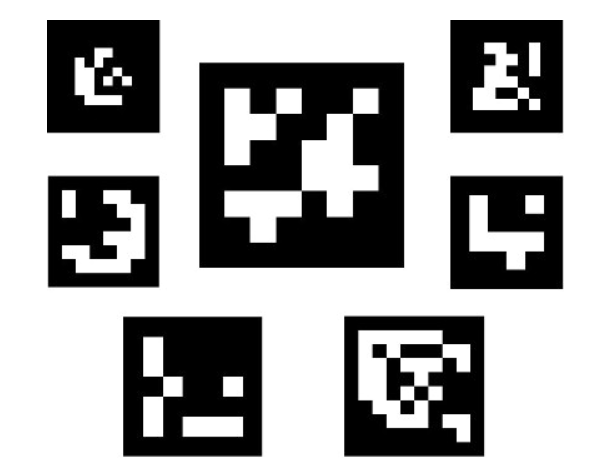
\includegraphics[scale=0.5]{marker_img.PNG} 
\caption{Esempio di immagini dei marcatori}
\end{figure}

Va notato che un marcatore può essere trovato ruotato nell'ambiente, tuttavia, il processo di rilevamento deve essere in grado di determinare la sua rotazione originale, in modo che ogni angolo sia identificato inequivocabilmente. Questo viene fatto anche in base alla codifica binaria.

Un dizionario di marcatori è un insieme di marcatori considerati in un'applicazione specifica. È semplicemente la lista delle codifiche binarie di ciascuno dei suoi marcatori.

Le proprietà principali di un dizionario sono la dimensione del dizionario(il numero di marcatori) e la dimensione del marcatore(le dimensione effettive del marcatore).
\paragraph{Reindirizzamento topic}
Precedentemente lo \textit{Star-marker-finder} utilizzava una camera usb per localizzare i marcatori e dedurre la propria posizione. Adesso al posto del nodo della camera usb viene utilizzato il nodo della ZED.
Bisogna modificare i file lunch dello star-marker-finder, si trova nel percorso
\begin{verbatim}
\ROS\src\star_marker_finder\launch
\end{verbatim}
E cambiare le voci di \textit{remap}, è sufficiente scegliere una delle due camera sinistra o destra.
\begin{verbatim}
    <remap from="image_rect" to="/left/image_rect_color"/>
    <remap from="camera_info" to="/left/camera_info"/>
\end{verbatim}

\subsection{Marker-finder su architettura distribuita}
Il programma è stato realizzato con l'obiettivo di rendere autonoma la guida di un robot esistente. 
Quest'ultimo è dotato di un computer di bordo responsabile del movimento delle quattro ruote omnidirezionali connesse attraverso un cavo RJ45.
Si è voluto implementare la comunicazione tra questo pc e la scheda Jetson in modo da separare la parte di gestione della locomozione da quella di odometria e elaborazione dati.
La connessione tra i due calcolatori è stata effettuata attraverso un ulteriore cavo rj45 in configurazione crossover, creando una rete LAN.
È risultato necessario assegnare un ip statico alle due interfacce di rete, configurabile tramite il network-manager di ubuntu o con un semplice comando da terminale:
\begin{verbatim}
ifconfig eth0 192.168.0.2 netmask 255.255.255.0 up
\end{verbatim}
In questo caso si presuppone che la porta ethernet sia riconosciuta dal sistema come "eth0" mentre l'indirizzo ip è un indirizzo ip scelto casualmente.Per l'indirizzo ip del secondo pc si tenga conto della convenzione adottata nel primo ovvero, in questo caso, 24 bit di subnet e 8 di indirizzamento (l'ip della seconda scheda dovrà essere del tipo 192.168.0.x ).
Una volta stabilita la connessione, confermata generalmente da una notifica desktop di sistema, bisogna effettuare il setup dei terminali utilizzati per ROS.
In un sistema distribuito roscore viene eseguito su di una sola macchina, alle altre macchine connesse viene fornito l'ip della macchina che sta eseguendo roscore in modo da poter connettere i propri nodi ad esso.


















\newpage
\section{eProsima DDS}

Il Data Distribution Service for Real Time Systems (DDS) è uno standard emanato dall'Object Management Group (OMG) che definisce un middleware per la distribuzione di dati in tempo reale secondo il paradigma publish/subscribe.
Il Data Distribution Service è concepito come una soluzione infrastrutturale alla programmazione di applicazioni incentrate sui dati. Il suo scopo è di nascondere interamente le problematiche della gestione della comunicazione nella programmazione di applicazioni data-centric.

\subsection{ROS 2}
L'obiettivo è di rendere DDS un dettaglio di implementazione di ROS 2.0. Ciò significa che tutte le API specifiche di DDS e le definizioni dei messaggi devono essere nascoste. DDS offre funzionalità di rilevamento, definizione dei messaggi, serializzazione dei messaggi e trasporto di pubblicazione-sottoscrizione. Pertanto, DDS fornirebbe la scoperta, il trasporto di pubblicazione-sottoscrizione e almeno la serializzazione del messaggio sottostante per ROS. ROS 2.0 fornirà un'interfaccia ROS 1.x simile a DDS che nasconde gran parte della complessità di DDS per la maggior parte degli utenti di ROS, ma fornisce  separatamente l'implementazione DDS sottostante per gli utenti che hanno casi di utilizzo estremi o necessità di integrarsi con altri sistemi DDS esistenti.

\begin{figure}[htbp]
\centering
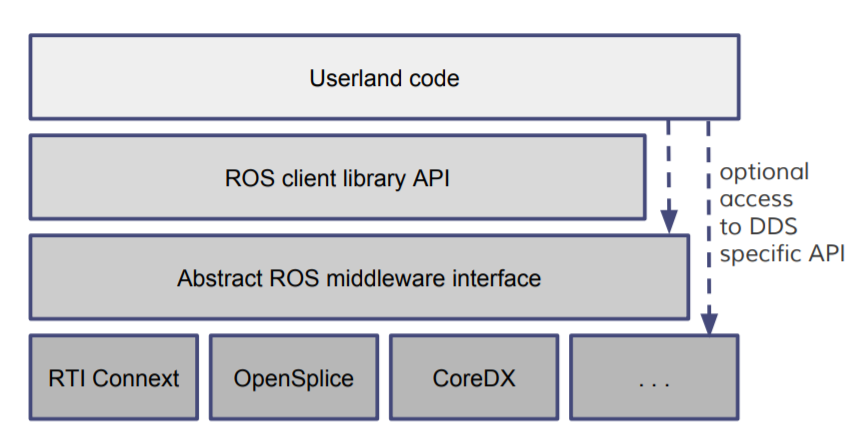
\includegraphics[scale=0.5]{dds_img.PNG} 
\caption{Layout API DDS e ROS}
\end{figure}


L'accesso all'implementazione DDS richiederebbe a seconda di un pacchetto aggiuntivo che non viene normalmente utilizzato. In questo modo puoi capire se un pacchetto si è legato a un particolare fornitore DDS semplicemente osservando le dipendenze del pacchetto. L'obiettivo dell'API ROS, che è in cima al DDS, dovrebbe essere quello di soddisfare tutte le esigenze comuni della comunità ROS, perché una volta che un utente accede al sistema DDS sottostante, perderà la portabilità tra i fornitori DDS. La portabilità tra i fornitori DDS non è intesa a incoraggiare le persone a scegliere frequentemente fornitori diversi, ma piuttosto a consentire agli utenti esperti di selezionare l'implementazione DDS che soddisfa i loro requisiti specifici, nonché a ROS a prova di futuro contro le modifiche nelle opzioni del fornitore DDS.

DDS sostituirà completamente il sistema di rilevamento basato sul master ROS. ROS dovrebbe attingere all'API di DDS per ottenere informazioni come un elenco di tutti i nodi, un elenco di tutti gli topics e il modo in cui sono connessi. L'accesso a queste informazioni sarebbe nascosto dietro una API definita ROS, impedendo agli utenti di dover chiamare direttamente in DDS.

\subsection{eProsima}
Il protocollo DDSI-RTPS (DDS-Interoperability Real Time Publish Subscribe) sostituirà i protocolli ROSRO TCPROS e UDPROS per i protocolli publish/subscribe.
\textit{Prosima Fast RTPS} è un'implementazione relativamente nuova, leggera e open source di RTPS. Consente l'accesso diretto alle impostazioni e alle caratteristiche del protocollo RTPS, il che non è sempre possibile con altre implementazioni DDS. 
Nella parte superiore di RTPS, troviamo il dominio, che definisce un piano separato di comunicazione. Diversi domini possono coesistere contemporaneamente in modo indipendente. Un dominio contiene un numero qualsiasi di partecipanti, elementi in grado di inviare e ricevere dati. Per fare ciò, i partecipanti usano i loro endpoint:

\begin{figure}[htbp]
\centering
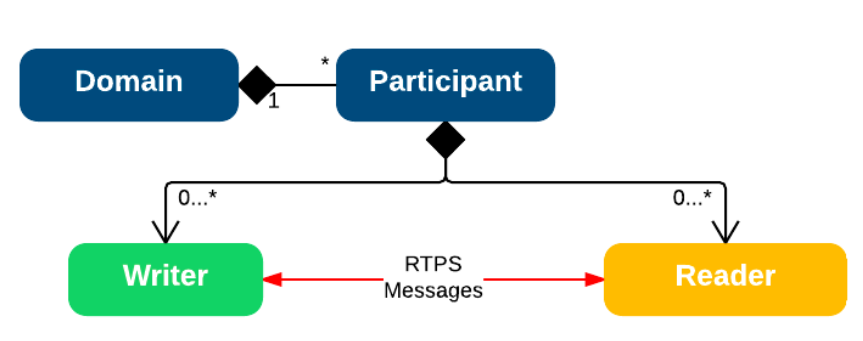
\includegraphics[scale=0.5]{dds_img1.PNG} 
\caption{Layout API DDS e ROS}
\end{figure}

\begin{itemize}
\item Reader: endpoint in grado di ricevere dati.

\item Writer: Endpoint in grado di inviare dati.
\end{itemize}

Un partecipante può avere un numero qualsiasi di scrittori e lettori endpoint.
La comunicazione ruota intorno ai Topics, che definiscono i dati scambiati. I Topics non appartengono ad alcun partecipante in particolare; invece, tutti i partecipanti interessati tengono traccia delle modifiche ai dati dell'argomento e si assicurano di tenersi aggiornati reciprocamente
\subsection{installazione}
eProsima ha bisogno di due componenti:
\begin{itemize}
\item eProsima RPC su DDS
\item eProsima Fast RTPS
\end{itemize}

Disponibili sul sito \href{https://www.eprosima.com/}{eProsima}.
\paragraph{eProsima RPC su DDS}
eProsima RPC su DDS richede l'installazione della libreria \textit{eProsima FastCDR}. La libreria eProsima FastCDR si trova sotto la cartella
\textit{"requiredcomponents"}. Bisogna estrarre il contenuto del pacchetto \textit{"eProsima-FastCDR-1.0.6-Linux.tar.gz"}
ed eseguire sul terminale:
\begin{verbatim}
For 32-bit machines

     cd eProsima_FastCDR-1.0.6-Linux;
     ./configure --libdir=/usr/lib;
     make; 
     make install
     
For 64-bit machines

    cd eProsima_FastCDR-1.0.6-Linux; 
    ./configure --libdir=/usr/lib64;
    make;
    make install
\end{verbatim}
richiede anche l'installazione della libreria \textit{eProsima FastRTPS} su
il tuo sistema. La libreria \textit{eProsima FastRTPS} viene fornita nella cartella
\textit{"requiredcomponents"}. Estrarre il contenuto del pacchetto
\textit{"eProsima-FastRTPS-1.3.1-Linux.tar.gz"} ed eseguire:

\begin{verbatim}
For 32-bit machines

    cd eProsima_FastRTPS-1.3.1-Linux; 
    ./configure --libdir=/usr/lib;
     make; 
     make install

For 64-bit machines

    cd eProsima_FastRTPS-1.3.1-Linux;
    ./configure --libdir=/usr/lib64;
    make;
    make install

\end{verbatim}

eProsima RPC su DDS richiede anche librerie \textit{Boost}. Se non sono presenti sulla macchina dovranno essere installati utilizzando il  Gestore dei pacchetti di Linux.
Installazione  eProsima RPC su DDS.

\begin{verbatim}
For 32-bit machines

    cd eProsima_RPCDDS-1.0.3-Linux;
    ./configure --libdir=/usr/lib;
    make;
    make install

For 64-bit machines

    cd eProsima_RPCDDS-1.0.3-Linux;
    ./configure --libdir=/usr/lib64;
    make;
    make install
\end{verbatim}

\paragraph{eProsima Fast RTPS}
Successivamente eProsima Fast RTPS richede l'installazione della libreria \textit{eProsima FastCDR} per eseguire alcuni degli esempi forniti e compilare il codice generato con \textit{eProsima FASTRTPSGEN}.
La libreria eProsima FastCDR è disponibile nella cartella \textit{"requiredcomponents"}. Estrare il contenuto del pacchetto \textit{"eProsima-FastCDR-1.0.7-Linux.tar.gz"} ed eseguire:
\begin{verbatim}
cd eProsima_FastCDR-1.0.7-Linux;
./configure --libdir=/usr/lib;
make;
sudo make install
\end{verbatim}
Installare il software eProsima Fast RTPS.
\begin{verbatim}
cd eProsima_FastRTPS-1.5.0-Linux;
./configure --libdir=/usr/lib;
make;
sudo make install

\end{verbatim}




\end{document}